

%----------------------------------------------------------------------------------------
%	PACKAGES AND OTHER DOCUMENT CONFIGURATIONS
%----------------------------------------------------------------------------------------

\documentclass[xcolor=x11names,compress]{beamer}
\usepackage{graphicx}
\usepackage{subfig}
\usepackage{tikz}
\usetikzlibrary{decorations.fractals}

\useoutertheme[subsection=false,shadow]{miniframes}
\useinnertheme{default}
\usefonttheme{serif}
\usepackage{palatino}

\setbeamerfont{title like}{shape=\scshape}
\setbeamerfont{frametitle}{shape=\scshape}
\setbeamertemplate{caption}[numbered]

\setbeamercolor*{lower separation line head}{bg=DeepSkyBlue4}
\setbeamercolor*{normal text}{fg=black,bg=white} 
\setbeamercolor*{alerted text}{fg=red} 
\setbeamercolor*{example text}{fg=black} 
\setbeamercolor*{structure}{fg=black} 
 
\setbeamercolor*{palette tertiary}{fg=black,bg=black!10} 
\setbeamercolor*{palette quaternary}{fg=black,bg=black!10} 

\addtobeamertemplate{navigation symbols}{}{%
    \usebeamerfont{footline}%
    \usebeamercolor[fg]{footline}%
    \hspace{1em}%
    \insertframenumber/\inserttotalframenumber
}

\renewcommand{\(}{\begin{columns}}
\renewcommand{\)}{\end{columns}}
\newcommand{\<}[1]{\begin{column}{#1}}
\renewcommand{\>}{\end{column}}




\begin{document}


%----------------------------------------------------------------------------------------
%	TITLE SECTION 
%----------------------------------------------------------------------------------------

\begin{frame}
\title{Impact of memory allocation on the performance of a delegation synchronization algorithm}
\author
{
	Presented by \textbf{SID-LAKHDAR Riyane}\\
    (M1 MoSIG: ENSIMAG / UJF)\\
	Directed by \textbf{ROPARS Thomas}\\
    (LIG, team ERODS)\\
	
\includegraphics[height=1cm,width=2cm]{logo/logoINP.png}
	
\includegraphics[height=1cm,width=2cm]{logo/logoUJF.jpg}
	
\includegraphics[height=1cm,width=1cm]{logo/logoLIG.jpg}
}
\date
{
	\vspace{1cm}
	\today
}
\titlepage
\end{frame}


%----------------------------------------------------------------------------------------
%	MOTIVATION
%----------------------------------------------------------------------------------------

\begin{frame}{Motivation: the multithreading limitation}
	\begin{figure}
		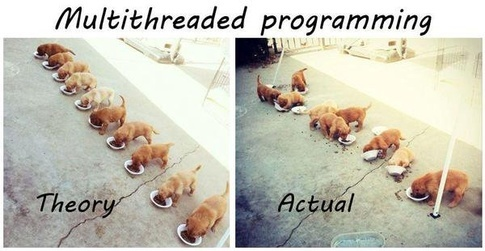
\includegraphics[width=0.7\linewidth]{charts/multithreading_theory_reality.jpeg}
	\end{figure}

	\begin{itemize}
		\item Theoretical objective of multithreading:
			\begin{equation*}
				Time(\mbox{multithreaded task}) = \frac{Time(\mbox{Sequential task})}{\mbox{Number of thread}}
			\end{equation*}

		\item Objective is still way of the mark
	\end{itemize}
\end{frame}


%----------------------------------------------------------------------------------------

\begin{frame}{Motivation: Complex processor $\rightarrow$ complex allocator}
	\begin{figure}[t]
	\begin{center}
		\subfloat
	    {
			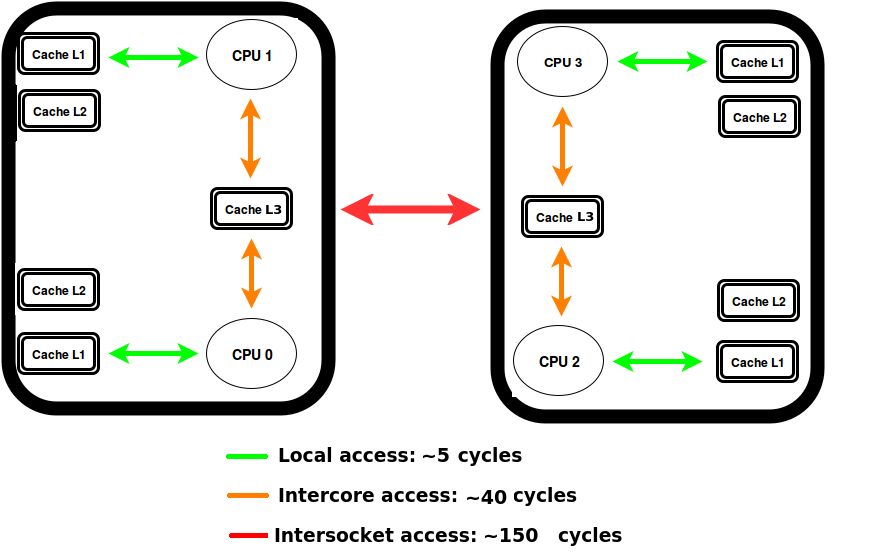
\includegraphics[width=0.8\linewidth]{charts/numaNode.png}
		}
	\end{center}
	\end{figure}

	\begin{itemize}
		\item \textbf{Memory allocator} is an important cause of this limitation
	\end{itemize}
\end{frame}


%----------------------------------------------------------------------------------------

\begin{frame}{Motivation: delegation approach}
	\begin{figure}[t]
	\begin{center}
		\subfloat
	    {
			\includegraphics[width=0.9\linewidth]{charts/delegationVsLock.png}
		}
	\end{center}
	\end{figure}
\end{frame}


%----------------------------------------------------------------------------------------

\begin{frame}{Our contribution}
	Prove the impact of dynamic  memory allocation on
	\begin{itemize}
		\item The absolute performances of multithreading
		\item The relative performance of two custom delegation algorithms
	\end{itemize}
\end{frame}


%----------------------------------------------------------------------------------------

\section{\scshape The delegation approach for mutual exclusion}
\frame{\tableofcontents}








%----------------------------------------------------------------------------------------
%	THE DELEGATION APPROACH
%----------------------------------------------------------------------------------------

\begin{frame}{The delegation approach}
	\begin{figure}[t]
	\begin{center}
		\subfloat
	    {
			\includegraphics[width=0.5\linewidth]{charts/delegationApproach.png}
		}
	\end{center}
	\end{figure}

	\begin{itemize}
		\item \textbf{Improve cache locality}: memory access of the CS are mostly locals
	\end{itemize}
\end{frame}


%----------------------------------------------------------------------------------------

\begin{frame}{The combiner algorithm}
	\begin{figure}[t]
	\begin{center}
		\subfloat
		{
			\includegraphics[width=0.5\linewidth]{charts/combinerAlgorithm.png}
		}
	\end{center}
	\end{figure}
\end{frame}


%----------------------------------------------------------------------------------------

\begin{frame}{The expected optimization: streaming store}
	\begin{figure}[t]
	\begin{center}
		\subfloat
		{
			\includegraphics[width=0.6\linewidth]{charts/delegationStreamingStore.png}
		}
	\end{center}
	\end{figure}
\end{frame}


%----------------------------------------------------------------------------------------

\begin{frame}{Limit of the evaluation: the allocator}
	\textbf{Used allocator}: 
	\begin{itemize}
		\item Large thread-local buffer used for all the allocations
		\item No returned memory
	\end{itemize}

	\textbf{Unrealistic allocator}: 
	\begin{itemize}
		\item Outperforms the general purpose allocators
        \item Cannot scale (memory footprint)
	\end{itemize}
\end{frame}


%----------------------------------------------------------------------------------------

\section{\scshape Memory allocation: challenges and proposed solutions}
\frame{\tableofcontents[currentsection]}










%----------------------------------------------------------------------------------------
%	MEMORY ALLOCATION: CHALLENGES AND PROPOSED SOLUTIONS
%----------------------------------------------------------------------------------------

\begin{frame}{Memory allocator:  thread-central bottleneck}
	\begin{figure}
		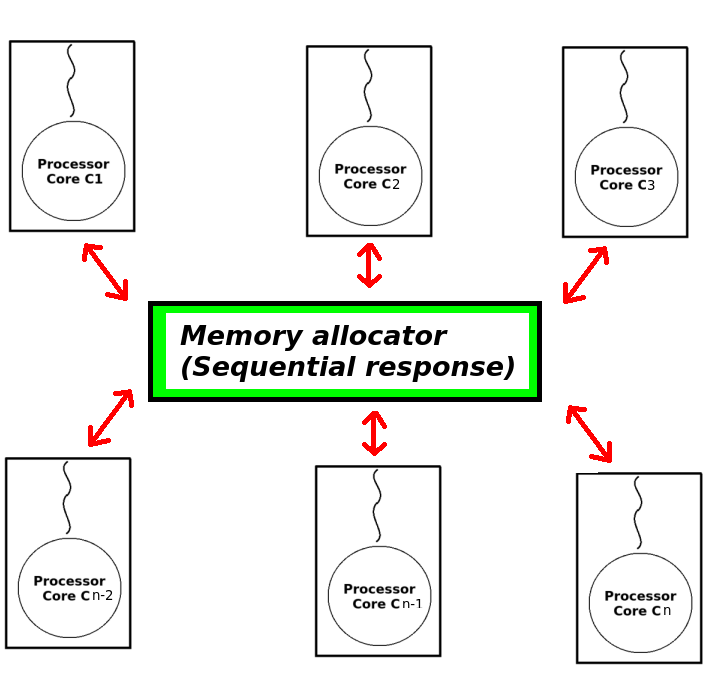
\includegraphics[width=0.5\linewidth]{charts/bottleneck.png}
	\end{figure}

	\begin{itemize}
		\item Sequential memory allocation
        \item Inefficient response to contention
	\end{itemize}
\end{frame}


%----------------------------------------------------------------------------------------

\begin{frame}{Core local buffer}
	\begin{figure}
		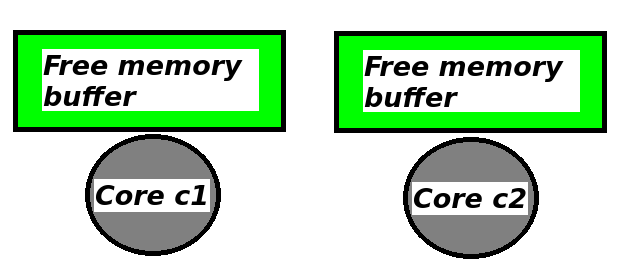
\includegraphics[width=0.7\linewidth]{charts/coreLocalBuffer.png}
	\end{figure}


	\begin{itemize}
		\item \textbf{Improved allocation time}
		\item \textbf{Buffer made of contiguous addresses} $\rightarrow$ low page-fault probability

	\end{itemize}
\end{frame}


%----------------------------------------------------------------------------------------

\begin{frame}{Further contention lightening}
	\begin{figure}
		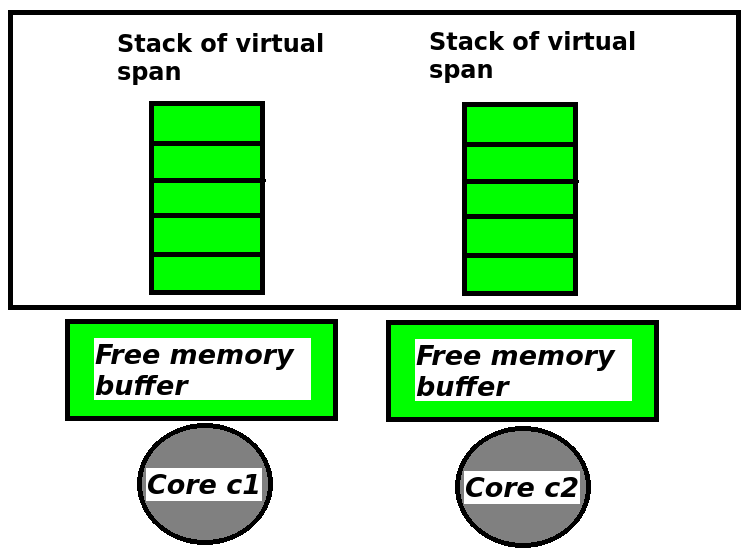
\includegraphics[width=0.6\linewidth]{charts/globalArchitecture.png}
	\end{figure}

	\textbf{One stack per core:}
	\begin{itemize}
		\item No synchronization between cores
		\item Lock free concurrent data structure
	\end{itemize}
\end{frame}


%----------------------------------------------------------------------------------------

\begin{frame}{Software issues: False sharing}
	\begin{figure}
		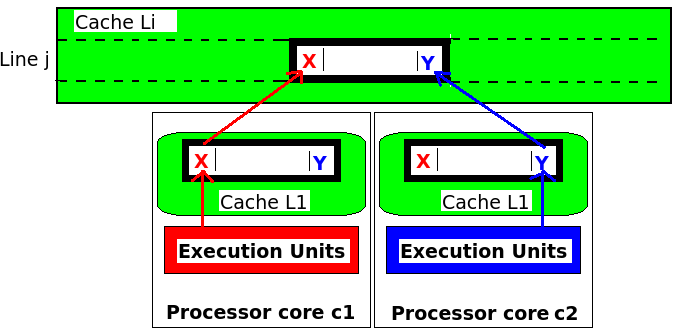
\includegraphics[width=1.0\linewidth]{charts/falseSharing.png}
	\end{figure}
\end{frame}


%----------------------------------------------------------------------------------------

\begin{frame}{The span structure}
	\begin{itemize}
		\item \textbf{Span size is a multiple of a cache line size:} no false sharing
        \item \textbf{Simplified allocation algorithm}
		\item \textbf{Extra memory aligned to page size:} swapped out of the RAM
	\end{itemize}
\end{frame}


%----------------------------------------------------------------------------------------

%\begin{frame}{Software issues: heavy processes}
%	\begin{itemize}
%		\item Switch from user to kernel mode
%		\item Internal and external fragmentation
%		\item Memory blowup
%	\end{itemize}
%\end{frame}










%----------------------------------------------------------------------------------------

\section{\scshape Experimental evaluations}
\frame{\tableofcontents[currentsection]}





%----------------------------------------------------------------------------------------
%	TESTING AND RESULTS . TESTING ENVIRONMENT
%----------------------------------------------------------------------------------------

\begin{frame}{Designed test environment}
	Two main rules: Avoid overhead linked to \textbf{scheduling}
	\begin{itemize}
		\item \textbf{No more threads than cores}
		\item \textbf{Pin threads on independent cores}
	\end{itemize}

	\bigskip

	Environments
	\begin{itemize}
		\item Processor \textbf{Intel Xeon E5-2620} with a \textbf{Debian} kernel 3.16.7
		\item Processor \textbf{AMD Opteron 6164} with a \textbf{Debian} kernel 3.16.7
	\end{itemize}

\end{frame}


%----------------------------------------------------------------------------------------

\begin{frame}{Testbed}
	Tested algorithms:
    \begin{itemize}
		\item Compare contention on a \textbf{Michael Scott} queue
        \item Compare the \textbf{combiner} and the \textbf{server based} algorithms.
	\end{itemize}

	\bigskip

	Considered memory allocators:
	\begin{itemize}
		\item \textbf{Custom allocator} (used in previous delegation evaluation)
        \item \textbf{ptmalloc} (C standard library)
        \item \textbf{hoard}
        \item \textbf{jemalloc}
        \item \textbf{scalloc}
        \item \textbf{supermalloc}
        \item \textbf{tcmalloc}
	\end{itemize}
\end{frame}




%----------------------------------------------------------------------------------------
%	TEST AND RESULTS
%----------------------------------------------------------------------------------------

\begin{frame}{Allocator comparison (with the combiner algorithm)}
	Compare the throughput of the \textbf{allocators}: The higher the better
	\begin{figure}[t]
    \begin{center}
		\subfloat[Intel Xeon E5-2620]{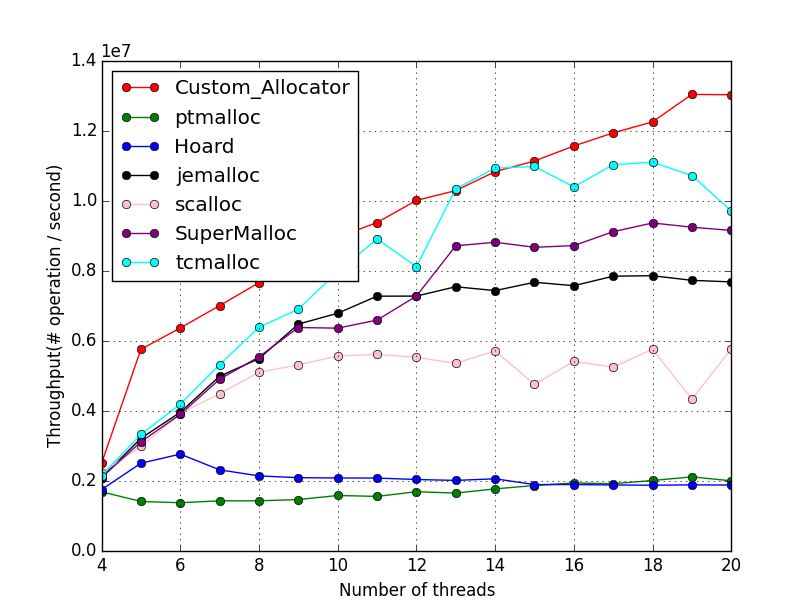
\includegraphics[width=0.5\linewidth]{chartsAllocator/20-Intel_Xeon_E5_2620-noOption-0-cc-msqueue.png}}
		\subfloat[AMD Opteron 6164]{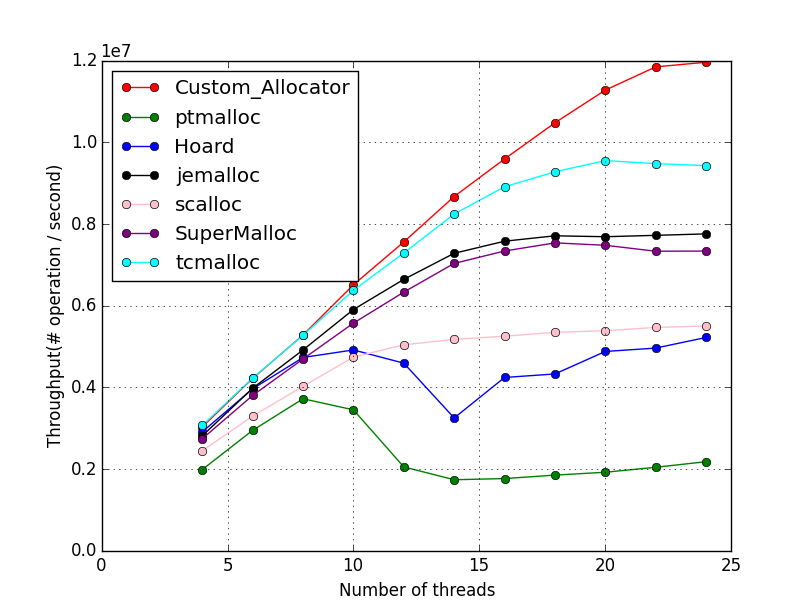
\includegraphics[width=0.5\linewidth]{chartsAllocator/24-AMD_Opteron_6164_HE-noOption-0-cc-msqueue}}
	\end{center}
	\end{figure}

	tcmalloc outperforms the general purpose allocators
\end{frame}


%----------------------------------------------------------------------------------------

\begin{frame}{Delegation algorithms comparison}
	Compare the throughput of the \textbf{delegation algorithms}: The higher the better

	\begin{figure}[t]
    \begin{center}
		\subfloat[Intel Xeon E5-2620]{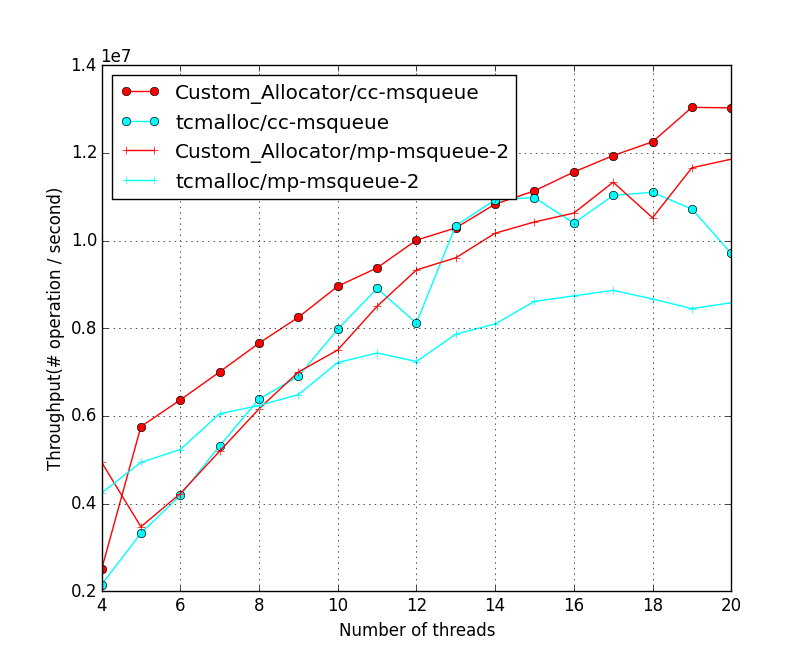
\includegraphics[width=0.5\linewidth]{chartsAllocator/20-Intel_Xeon_E5_2620-noOption-0-cc-msqueue+350-mp-msqueue-2-tcmalloc+Custom_Allocator.png}}
		\subfloat[AMD Opteron  6164]{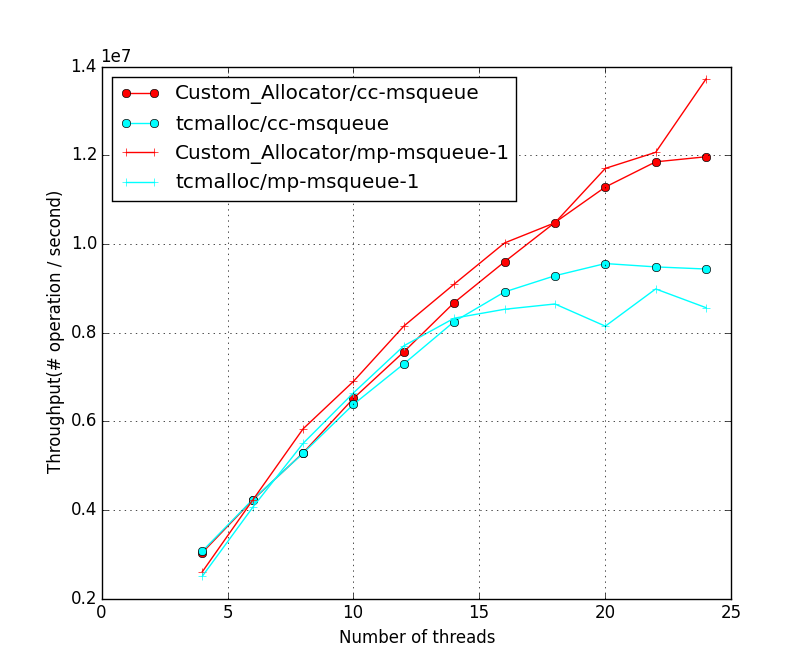
\includegraphics[width=0.5\linewidth]{chartsAllocator/24-AMD_Opteron_6164_HE-noOption-0-cc-msqueue+400-mp-msqueue-1-tcmalloc+CustomAllocator.png}}
	\end{center}
	\end{figure}

	Optimization property infirmed
\end{frame}




%----------------------------------------------------------------------------------------
%	RECAP
%----------------------------------------------------------------------------------------

\begin{frame}{Recap}
During this study, we have:
	\begin{itemize}
    	\item Highlighted the impact of memory allocation on multithreaded algorithms
        \item Infirmed the performance property of two delegation algorithms
	\end{itemize}

Open issues: understand the reasons of the noticed behavior
	\begin{itemize}
		\item The allocation design of tcmalloc
        \item The processor NUMA architecture policy
	\end{itemize}
\end{frame}



%----------------------------------------------------------------------------------------
%	FINAL
%----------------------------------------------------------------------------------------

\begin{frame}
\title{Impact of memory allocation on the performance of a delegation synchronization algorithm}
\author
{
	Presented by \textbf{SID-LAKHDAR Riyane}\\
	(M1 MoSIG: ENSIMAG / UJF)\\
	Directed by \textbf{ROPARS Thomas}\\
    (LIG, team ERODS)\\
	
\includegraphics[height=1cm,width=2cm]{logo/logoINP.png}
	
\includegraphics[height=1cm,width=2cm]{logo/logoUJF.jpg}
	
\includegraphics[height=1cm,width=1cm]{logo/logoLIG.jpg}
}
\date
{
	\vspace{1cm}
	\today
}
\titlepage
\end{frame}



\end{document}
